\documentclass[
11pt,]{beamer}
\usepackage{booktabs}
\graphicspath{{Images/}{./}}
\usetheme{Madrid}
\usefonttheme{default}
\usepackage{palatino} 
\usepackage[default]{opensans}
\useinnertheme{circles}
\usepackage[english,russian]{babel}

\setbeamertemplate{caption}{\raggedright\insertcaption\par}

\title{Сигнал от темной материи, захваченной астрофизическими объектами} 
\author[]{Товстун А.А.}
\begin{document}	
	\begin{frame}
		\titlepage % Output the title slide, automatically created using the text entered in the PRESENTATION INFORMATION block above
	\end{frame}
	
	\begin{frame}
		\frametitle{Введение}
		Способы обнаружения темной материи (ТМ)
\begin{itemize}
	\item Прямые (низкофоновые эксперименты по обнаружению рассеяния)
	\item В ускорителях
	\item Косвенный метод --- детектирование потоков нейтрино
\end{itemize}
	\end{frame}

	\begin{frame}
		\frametitle{Задача}
		Цель --- получить ограничения исходя из нейтринного сигналаот аннигиляции частиц ТМ для неупругих сценариев.

Для этого считается на небесном теле (обычно Солнце) скорость захвата
$C$ и определяется число частиц и аннигиляционные потоки исходя из уравнения
\begin{equation*}
	\cfrac{d N}{dt} = C - E \cdot N - \Gamma N^2
\end{equation*}
$E$ --- темп испарения, $\Gamma$ --- аннигиляции
\begin{equation*}
	d N_{Ann} = \int{d^3\vec{v}d^3\vec{v}_1d^3\vec{r}f_{\chi}(\vec{v},\vec{r})f_{\chi}(\vec{v}_1,\vec{r})|\vec{v}-\vec{v}_1|d\sigma_{Ann}}
\end{equation*}



	\end{frame}

	\begin{frame}
		\frametitle{Неупругие сценарии}
		Неупругий процесс забирает часть энергии частицы, поэтому захват усиливается. 

Рассматривалось неупругое рассеяние с эмиссией фотона, электрона или возбуждением уровней. (Не дает существенного усиления)
\begin{equation*}
	\chi + N \rightarrow \chi + N + \gamma
\end{equation*}
\begin{equation*}
	\chi + H \rightarrow \chi + H^*
\end{equation*}
\begin{equation*}
	\chi + H \rightarrow \chi + p + e^-
\end{equation*}

	\end{frame}

	\begin{frame}
		\frametitle{Неупругая темная материя}
		Неупругая темная материя,состоящая из двух состояний $m_1$ и $m_2$ м небольшой разницей масс $\delta m$
\begin{equation*}
	m_1 \approx m_2 \approx m
\end{equation*}	
\begin{equation*}
	m_2 - m_1 = \delta m
\end{equation*}

Рассеяние на ядрах происходит с переходом
\begin{equation*}
	\chi + N \rightarrow \chi^* + N'
\end{equation*}	

	\end{frame}

	\begin{frame}
		\frametitle{Термализация}
		В двухкомпонентной ТМ происходит нетривиальная термализация. Для ее расчета рассматривается движение в сферическом потенциале.
\begin{equation*}	
	H = \frac{v_{r}^{2}}{2} + \left( {\phi(r) + \frac{L^{2}}{2r^{2}}} \right) = \frac{v_{r}^{2}}{2} + U_{eff}(L,r)
\end{equation*}
В уравнении Больцмана
\begin{equation*}
	\frac{df}{dt} = C\left( {\vec{r},\vec{v}} \right) + St \left[ f( \vec{r},\vec{v}')\right] \left( {\vec{r},\vec{v}} \right)
\end{equation*}
идет переход к параметрам $E,L$ - энергия и момент импульса.


	\end{frame}
	
	\begin{frame}
		\frametitle{Термализация}
		Мы будем решать линейное уравнение в матричном виде.
\begin{equation*}
	\frac{\partial \widetilde{f}_i}{\partial t} = \sum_j S_{ij}\widetilde{f}_j - \sum_j S_{ji} \widetilde{f}_i - E_i \widetilde{f}_i
\end{equation*}
где индексы $ij$ пробегают все состояния фазового пространства $E,L$.

Приближенное решение с шагом $\tau$:
\begin{equation*}
	\vec{\widetilde{f}}(t_n) = (1+\tau A)^n \vec{\widetilde{f}}(t_0),
	 \vec{\widetilde{f}}(t_0) = \vec{C}
\end{equation*}
Реальное распределение $f$ --- получается интегрированием функции $\widetilde{f}$ по времени.
\begin{equation*}
	f(t) = \int_0^t \widetilde{f} dt
\end{equation*}

	\end{frame}

	\begin{frame}
		\frametitle{Пример}
		Пример моделирования: $m=100GeV, \delta m = 10^{-4} GeV$
\begin{columns}[c]
	\begin{column}{0.5\textwidth} % Left column width
		\begin{figure}
				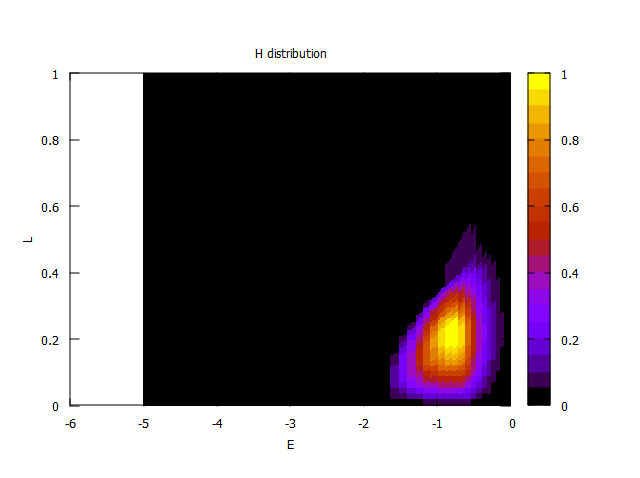
\includegraphics[width=\linewidth
				]{images/dh_100_dm.png}
				\caption{захват тяжелой компоненты}
		\end{figure}
	\end{column}
	\begin{column}{0.5\textwidth} 
		\begin{figure}
				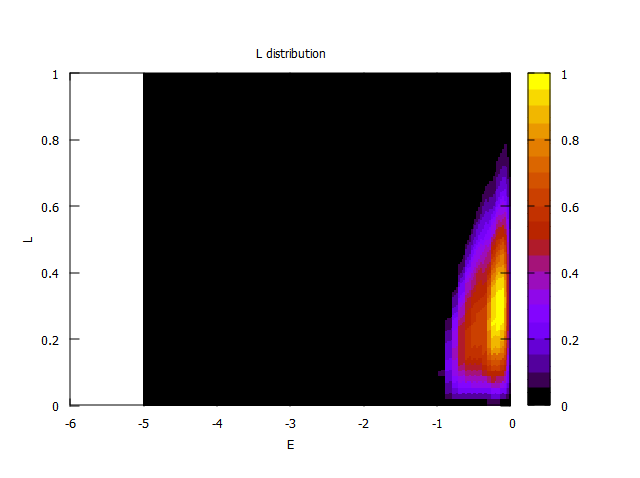
\includegraphics[width=\linewidth]
				{images/dl_100_dm.png}
				\caption{захват легкой компоненты}
		\end{figure}
	\end{column}
\end{columns}
	\end{frame}

%	\begin{frame}
%		\frametitle{Пример}
%		Конечное распределение
\begin{columns}[c]
	\begin{column}{0.5\textwidth} % Left column width
		\begin{figure}
			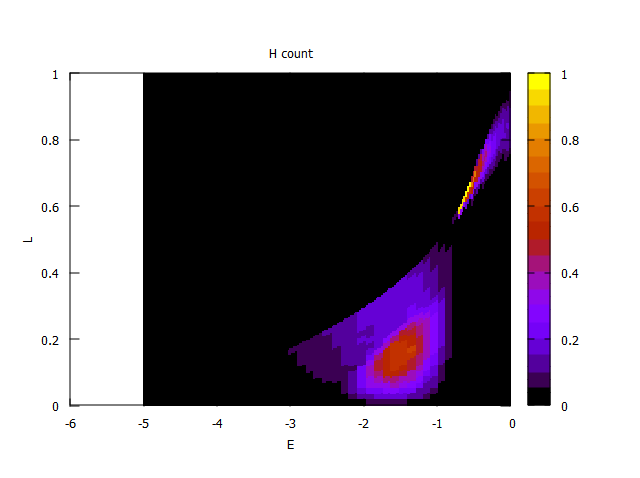
\includegraphics[width=\linewidth
			]{images/dhf.png}
			\caption{распределение тяжелой компоненты, $t = 2^{16}t_0$}
		\end{figure}
	\end{column}
	\begin{column}{0.5\textwidth} 
		\begin{figure}
			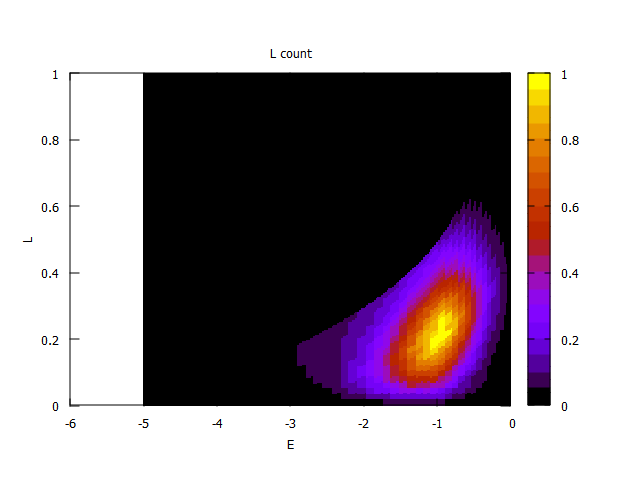
\includegraphics[width=\linewidth]
			{images/dlf.png}
			\caption{распределение легкой компоненты, $t = 2^{16}t_0$}
		\end{figure}
	\end{column}
\end{columns}
%	\end{frame}

	\begin{frame}
		\frametitle{Пример}
		Соотношение между компонентами (в качестве начального условия тяжелой в гало нет)
\begin{figure}
	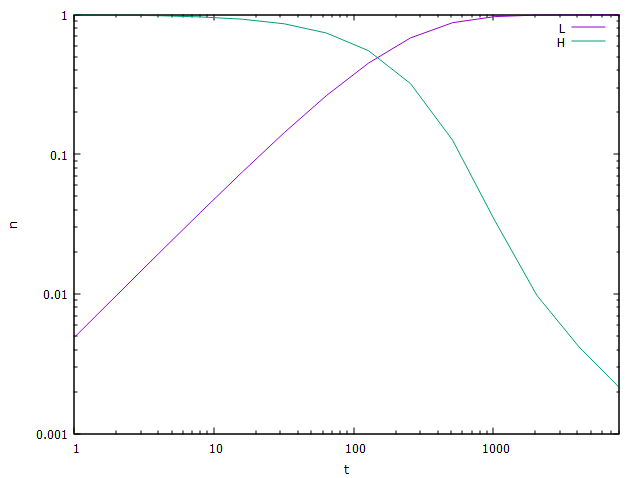
\includegraphics[width=0.7\linewidth]{images/evolution.png}
	\caption{Динамика числа частиц}
\end{figure}
	\end{frame}

	\begin{frame}
		\frametitle{Итоги}
		\begin{itemize}
	\item Показано, что для неупругих процессов вклад незначителен.
	\item Написана часть программы, которая находит захват, интеграл столкновений и считает эволюцию
	\item Осталось: Найти итоговое распеделение и потоки частиц.
\end{itemize}
	\end{frame}
	
	\begin{frame}
		\frametitle{Приложение}
		Скорость захвата определяется интегралом
\begin{equation*}
	C = \int{d^3\vec{v}d^3\vec{v}_i d^3\vec{r}f_{0\chi}(\vec{v},\vec{r})f_{i}(\vec{v}_i,\vec{r})|\vec{v}-\vec{v}_i|d\sigma}
\end{equation*}
где $f_{i}$ --- функция расределения ядер типа $i$, $f_{0\chi}$ --- распределение частиц пришедших из гало (с плотностью $0.3 GeV/cm^3$).
Предполагается гауссово распределение скоростей со сдвигом из-за  движения тела.
Интеграл столкновений в координатах $E,L$ следующий

\begin{equation*}
	dN = \int{dEdL \cfrac{T_{in}}{T_{in}+T_{out}} d\tau f_{0\chi}(E,L)f_{i} d^3\vec{v}_i(\vec{v}_i,\vec{r})|\vec{v}-\vec{v}_i|d\sigma}
\end{equation*}
Сетка по $E, L$ --- прямоугольная, неравномерная (число разбиений по $L$ зависит от $E$ ) 
	\end{frame}

\end{document} 

